%
%% Kapitel: Kapitel 4
%%======================================================================

\chapter{Zusammenfassung und Ausblick}
\label{cha:Zusammenfassung und Ausblick} \index{Zusammenfassung und Ausblick}
%
%
Ziel dieser Arbeit war es eine geeignete Simulationsumgebung f\"ur das Testen des Carolo-Cup-Fahrzeugs der Hochschule Karlsruhe zu finden und eine Fahrbahn nach Regeln des Carolo-Cups zu implementieren. Au{\ss}erdem sollten geeignete Bildverarbeitungsalgorithmen auf ihre Eignung getestet werden, welche anschlie{\ss}end zu einem funktionierenden Gesamtsystem kombiniert werden sollten.

Zur Umsetzung dieser Aufgabe wurde sich mit verschiedenen Simulationsumgebungen auseinandergesetzt und sich in die Simulationsumgebung Gazebo eingearbeitet. Die simulierte Fahrbahn wurde modular durch Pycairio und verschiedene Python-Skripte gestaltet. Alle m\"oglichen Fahrsituationen wurden als Bilddateien implementiert und lassen sich durch den Gazebo-Client von Hand in die Simulation einf\"ugen. Zudem wurde ein Fahrzeug mit Ackermann-Lenkung und zugeh\"origem Kamera-Plugin implementiert, welches die Dimension des echten Fahrzeugs besitzt und sich mit einem Controller steuern l\"asst. Bei der Programmierung in C++ wurde sich strikt an die Regeln des Google-Programming-Style-Guide gehalten. Tiefe Kenntnisse in Datenstrukturen wurden sich angeeignet und implementiert.
Verschiedene Algorithmen der Bildverarbeitung wurden n\"aher betrachtet und implementiert. Wie etwa ein Mittellinienclustering oder die Liniensuche durch den Hough-Lines-Algorithmus. Zudem wurde ein Bewertungsverfahren entwickelt das Fahrbahnbereiche mit einem Score bewertet. Auch wurden verschiedene Algorithmen implementiert die Hindernisse oder Markierungen auf der Fahrbahn detektieren und klassifizieren. Drei Methoden zur Klassifikation von Geschwindigkeitsbegrenzungsmarkierungen wurden ausgewertet, welche die Markierungen klassifizieren \"onnen. Zudem wurde ein Testframework implementiert, welches durch den modular aufgebauten Code ein Unit-Testing der Software erm\"oglicht.

Das Ergebnis dieser Arbeit ist ein robustes Bildverarbeitungssystem welche Au{\ss}en- und Mittellinien in Betracht zieht und Fahrbahnbereiche auf ihre Sicherheit auswertet und auch Objekte und Markierungen in der Fahrbahn detektieren kann. Zudem ist eine geeignete Simulationsumgebung entwickelt worden, um alle m\"oglichen Fahrsituationen des Carolo-Cups effizient testen zu k\"onnen.

\newpage

\begin{figure}[H]
\begin{center}
  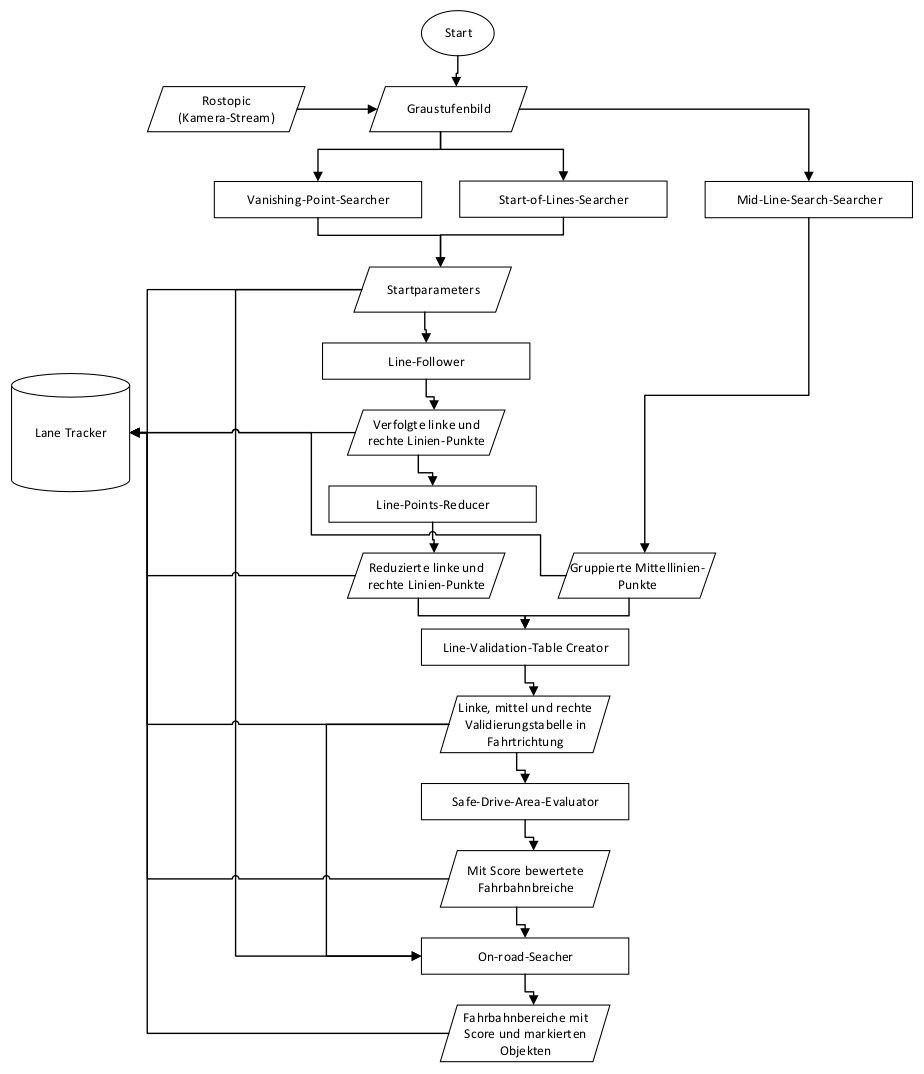
\includegraphics[width=1.1\textwidth]{/home/tb/gazebo_road_generation/02_Arbeit_Latex/012_Kapitel11/Bilder/gasamt_programm_finish1}% keine extention: wählt jpg für DVI
  \caption[gs]%
           {\label{fig:gs}%
           Programmablaufplan der Gesamtsoftware}
\end{center}
\end{figure}

\newpage


Im Laufe der Erstellung dieser Arbeit haben sich durch die gesammelten Erkenntnisse einige
Erweiterungsm\"oglichkeiten aufgetan:



\begin{itemize}
\item Beim Zusammenf\"uhren der Fahrbahnsegmente in der Simulation, sollte das Einstellen des Mittellinienoffsets automatisiert werden.

\item Die D\"ampfung des implementierten Fahrzeugs sollten an die des echten Fahrzeugs angepasst werden.

\item Die erzeugte Qt-GUI k\"onnte um weitere Features erweitert werden. Wie etwa dem Spawnen von Verkehrszeichen. 

\item Um eine bessere Performance der Bildverarbeitungsalgorithmen zu erm\"oglichen sollten die Verfahren parallelisiert werden.

\item Die M\"oglichkeit die Fahrspur zu wechseln kann implementiert werden, indem zur Laufzeit die Initialisierungsparameter angepasst werden.

\item Beim Mittellinienclustering sollte nicht jedes Pixel betrachtet werden, sondern in einer gewissen Schrittweite vorangeschritten werden um die Performance zu steigern.

\item Die Fahrbereichsbewertung sollte mit der Odometrie des Fahrzeugs gekoppelt werden, um so eine noch genauere Situationseinsch\"atzung zu erhalten.

\item Das Erkennen von Hindernissen und der Startboxschranke sollte mit den Time-of-Flight Sensoren abgeglichen werden.

\item Die sicheren Fahrbereiche des vorherigen Frames sollten mit dem aktuellen Frame verglichen werden, um noch eine bessere Sicherheitsbewertung zu erhalten.

\item Bei der Klassifikation der Geschwindigkeitsbegrenzungsmarkierungen sollte ein eigener Datensatz erzeugt werden, der auch eine Klasse enth\"alt in die Observationen fallen k\"onnen welche keine Markierungen sind. Da die Interklassenvarianz der verschiedenen Geschwindigkeitsmarkierungen sehr niedrig ist, sollten vielleicht auch weniger Klassen in betracht gezogen werden.

\end{itemize}



